\documentclass[aspectratio=169,11pt]{beamer}

\usetheme{Singapore}
\usepackage[utf8]{inputenc}
\usepackage{amsmath}
\usepackage{amsfonts}
\usepackage{amssymb}
\usepackage{graphicx}
\usepackage{hyperref}
\usepackage{booktabs}
\usepackage{listings}
\usepackage{xcolor}
\usepackage{caption}
\usepackage{subcaption}


% Define the settings for codechunks
\definecolor{codegreen}{rgb}{0,0.6,0}
\definecolor{codegray}{rgb}{0.5,0.5,0.5}
\definecolor{codepurple}{rgb}{0.58,0,0.82}
\definecolor{backcolour}{rgb}{0.9,0.9,0.9}
\lstdefinestyle{mystyle}{
    backgroundcolor=\color{backcolour},   
    commentstyle=\color{codegreen},
    keywordstyle=\color{magenta},
    numberstyle=\tiny\color{codegray},
    stringstyle=\color{codepurple},
    basicstyle=\ttfamily\footnotesize,
    breakatwhitespace=false,         
    breaklines=true,                 
    captionpos=b,                    
    keepspaces=true,                 
    numbers=left,                    
    numbersep=5pt,                  
    showspaces=false,                
    showstringspaces=false,
    showtabs=false,                  
    tabsize=2
}
\lstset{style=mystyle}

% Setup the bibliography
\usepackage[style=authortitle,backend=bibtex,citestyle=verbose]{biblatex}
\addbibresource{bibliography.bib}
\setbeamertemplate{bibliography item}[text]
\setbeamerfont{footnote}{size=\tiny}

% Allow footnotes with no number
\newcommand\blfootnote[1]{%
  \begingroup
  \renewcommand\thefootnote{}\footnote{#1}%
  \addtocounter{footnote}{-1}%
  \endgroup
}

% Allow section title slides
\AtBeginSection[]{
  \begin{frame}
  \vfill
  \centering
  \begin{beamercolorbox}[sep=8pt,center,shadow=true,rounded=true]{title}
    \usebeamerfont{title}\insertsectionhead\par%
  \end{beamercolorbox}
  \vfill
  \end{frame}
}

\author{Dr Stephen Pederson}
\title{Lecture 10: Single-Cell RNA Sequencing}
\subtitle{BIOINF3005/7160: Transcriptomics Applications}
%\setbeamercovered{transparent} 
\setbeamertemplate{navigation symbols}{} 
\logo{
	
\includegraphics[scale=0.3]{figures/UoA_logo_col_vert.png} 
} 
\institute{Bioinformatics Hub, \\The University of Adelaide} 
\date{May 25th, 2020} 
\subject{BIOINF3005/7160: Transcriptomics Applications} 


\begin{document}

\begin{frame}
\titlepage
\end{frame}

\begin{frame}
\footnotesize
\tableofcontents
\end{frame}


\section{Background}

\begin{frame}{Introduction}

	\begin{itemize}
		\item scRNA-Seq is the `latest and greatest' transcriptomic technique
		\item Previously all our analysis involved multiple cells per sample
		\item All were combined during tissue extraction, library preparation etc.
		\item Most experiments have \textbf{highly} heterogeneous cell populations, e.g.
		\pause
		\begin{itemize}
			\item Different regions of the brain contain highly specialised cells
			\item The immune system is highly complex
			\item Cancer samples have both infiltrating and tumour cells
		\end{itemize}
	\end{itemize}


\end{frame}

\begin{frame}{Introduction}

	\begin{itemize}
		\item If a gene is increased 2-fold in expression:
		\begin{itemize}
			\item Is this 2-fold in 100\% of cells?
			\item Or is it 4-fold in 50\% of cells?
			\item Or is it down 2-fold in 25\% and up 8-fold in 25\% and unchanged in 50\%?
		\end{itemize}
		\item Changes in gene expression can be highly specific to individual cell-types
		\item In general, determining heterogeneity of our samples is challenging
	\end{itemize}

\end{frame}

\begin{frame}{Introduction}

	\begin{itemize}
		\item The most intuitive solution is to obtain RNA from each cell and sequence
		\item Reality is much trickier than this
		\pause
		\item How do we characterise which cell is which cell-type?
		\item How do we capture as many transcripts from each cell as we can?
		\begin{itemize}
			\item Missing values are a huge issue in scRNA-seq
		\end{itemize}
		\item How do we compare within the same cell-types between experimental groups?
		\begin{itemize}
			\item E.g., treated and untreated cell types may not be assigned to the same cluster/cell-type
		\end{itemize}
	\end{itemize}

\end{frame}


\begin{frame}{Workflow Outline}

	\begin{center}
	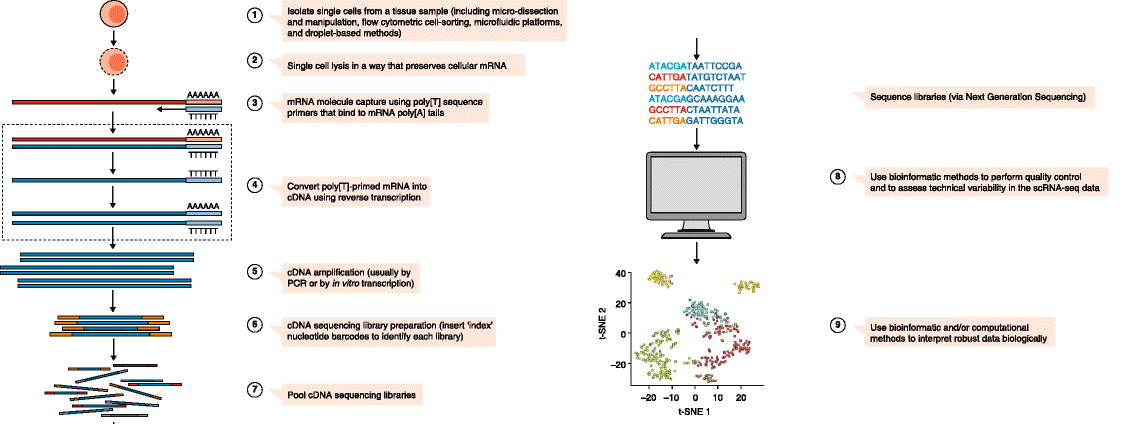
\includegraphics[width=0.27\textwidth]{figures/scRNAWorkflow.png} 
	\end{center}
	
	\blfootnote{Taken from \cite{pmid28821273}}

\end{frame}

\section{scRNA Protocols}

\subsection{Cell Isolation}

\begin{frame}{Isolating Individual Cells}

	\begin{itemize}
		\item Early protocols used a dilution series or manual isolation with a microscope (\textit{micromanipulation})
		\item Laser Capture Micro-dissection (LCM)
		\item Fluorescence-Activated Cell Sorting (FACS)
		\begin{itemize}
			\item Labelled antibodies to specific surface markers 
			\item MACS is a magnetic-based approach
		\end{itemize}
		\item Microfluidics/Droplet-based approaches
	\end{itemize}

\end{frame}

\begin{frame}{Protocol Timeline}

	\begin{center}
		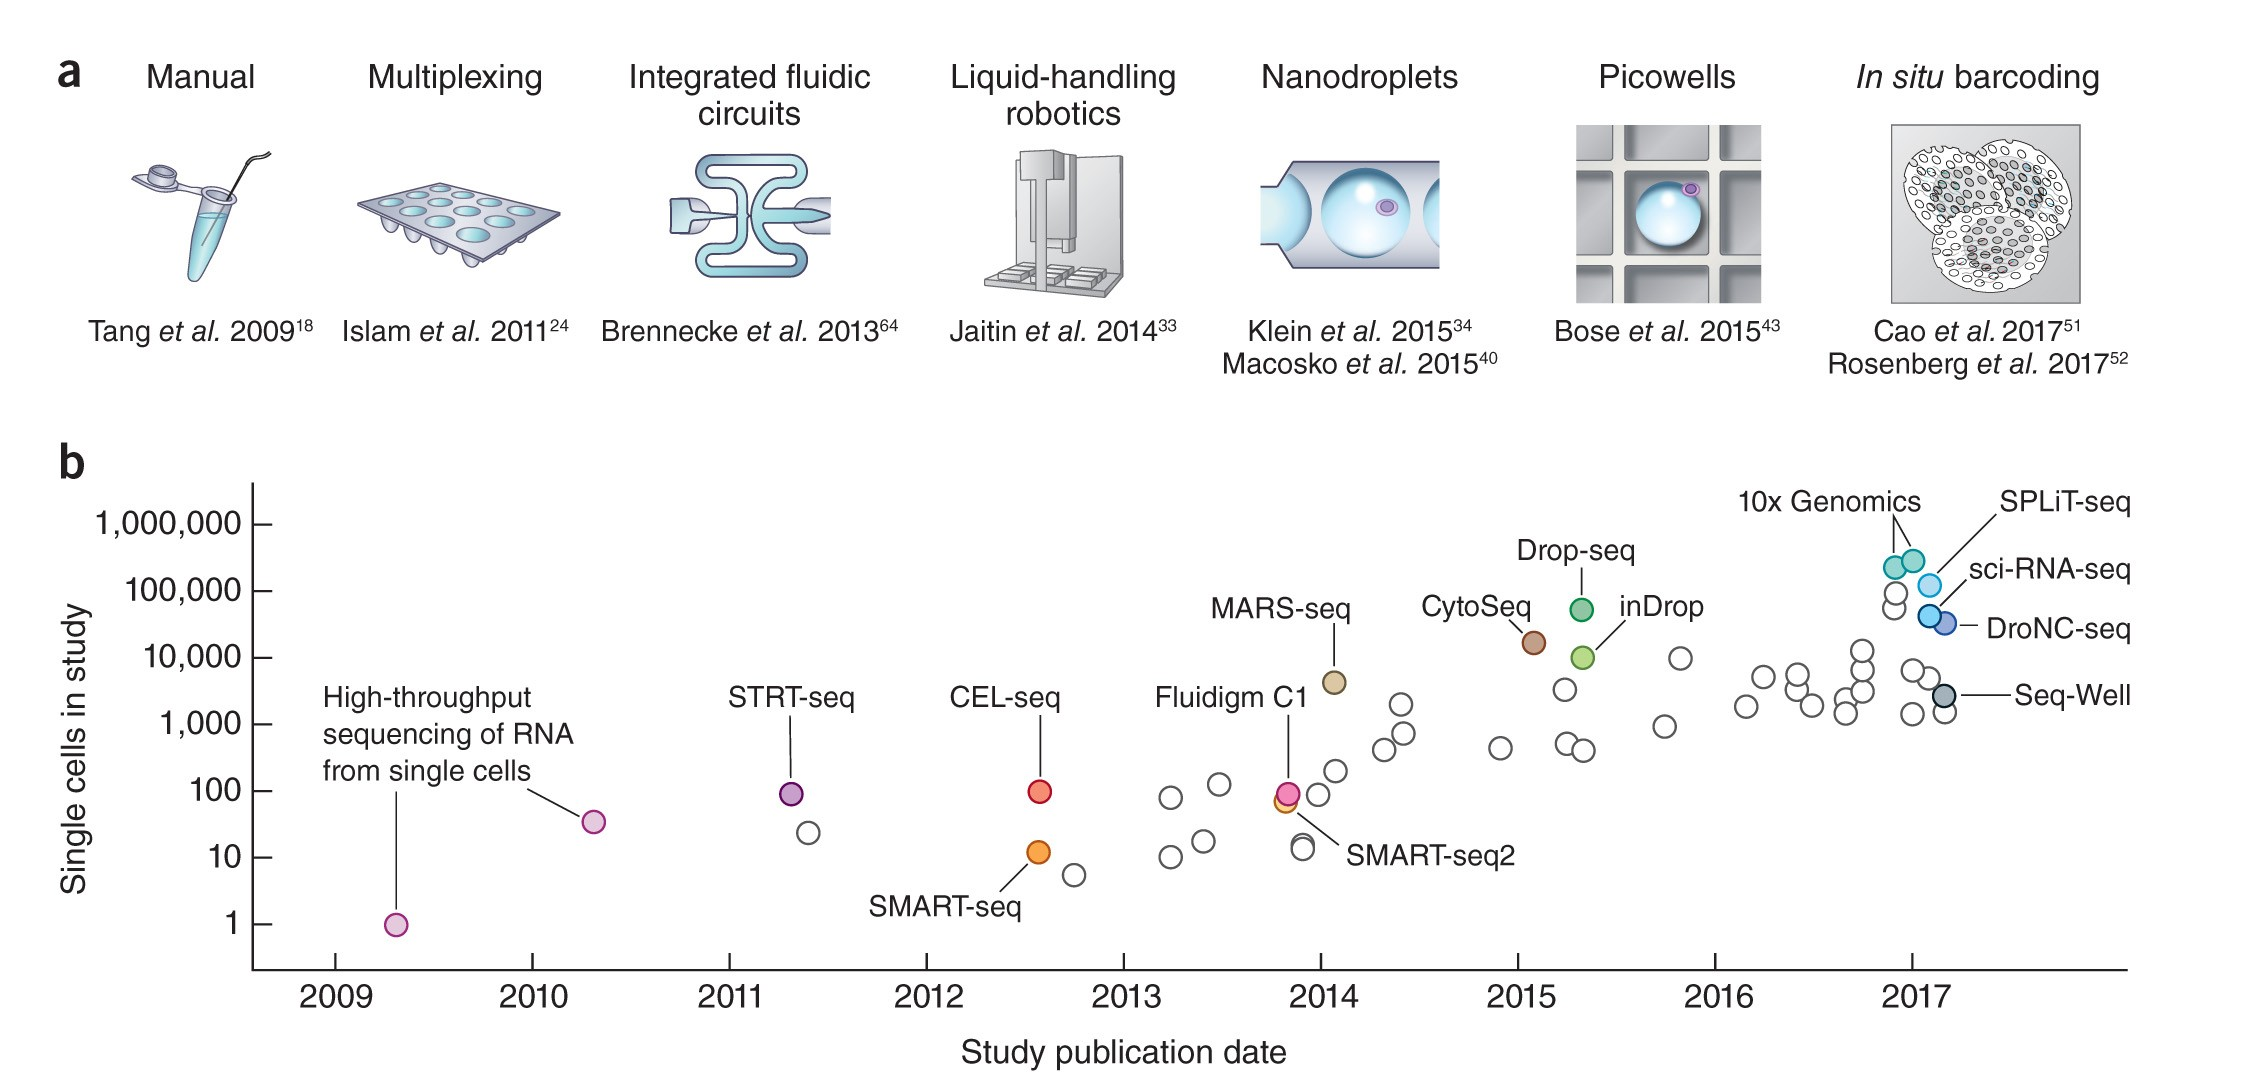
\includegraphics[width=0.85\textwidth]{figures/scRNATimeline.jpg} 
	\end{center}

	\blfootnote{Taken from \cite{pmid29494575}}

\end{frame}

\begin{frame}{Protocol Timeline}

	\begin{center}
		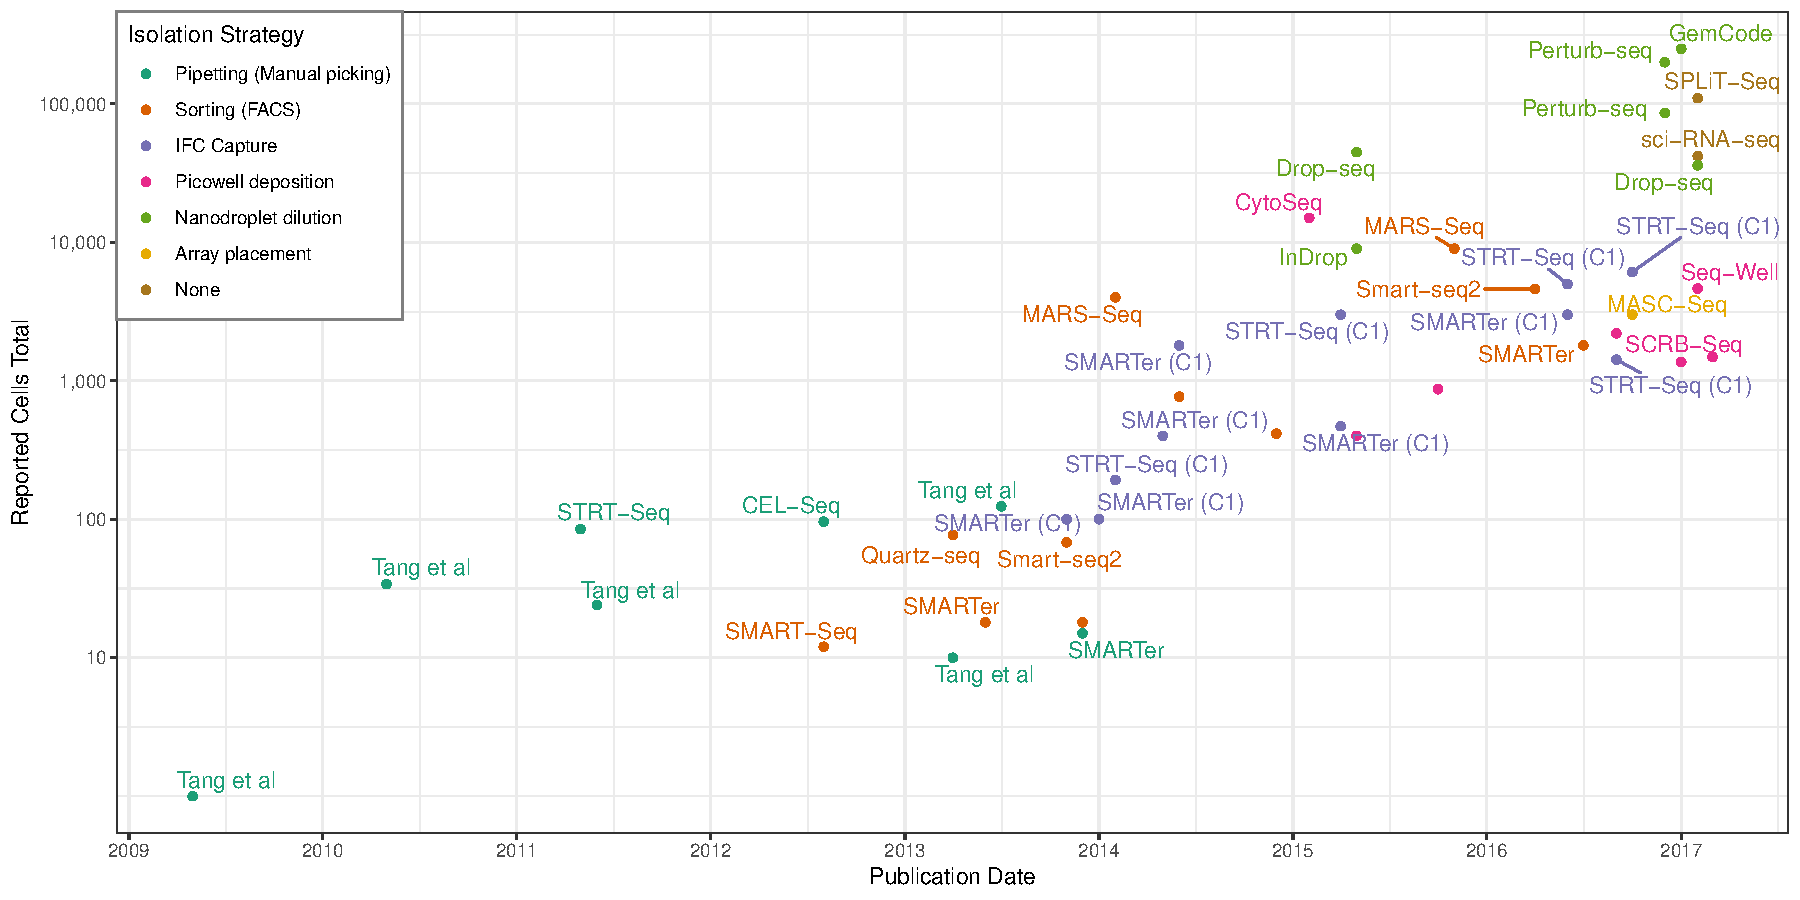
\includegraphics[width=0.85\textwidth]{figures/scRNATimeline.pdf} 
	\end{center}

	\blfootnote{Data taken from \cite{pmid29494575}}

\end{frame}

\begin{frame}{IFC Capture}

	\begin{itemize}
		\item Integrated Fluidic Circuit (IFC) chips
		\begin{itemize}
			\item Most common is the Fluidigm C1
		\end{itemize}
		\item Deliver tiny volumes into `reaction chambers'
		\item Early chips had 96 chambers $\implies$ multiple chips / experiment
		\item Recent chips handle $\sim$800 cells
	\end{itemize}

\end{frame}

\begin{frame}{Protocol Timeline}

	\begin{center}
		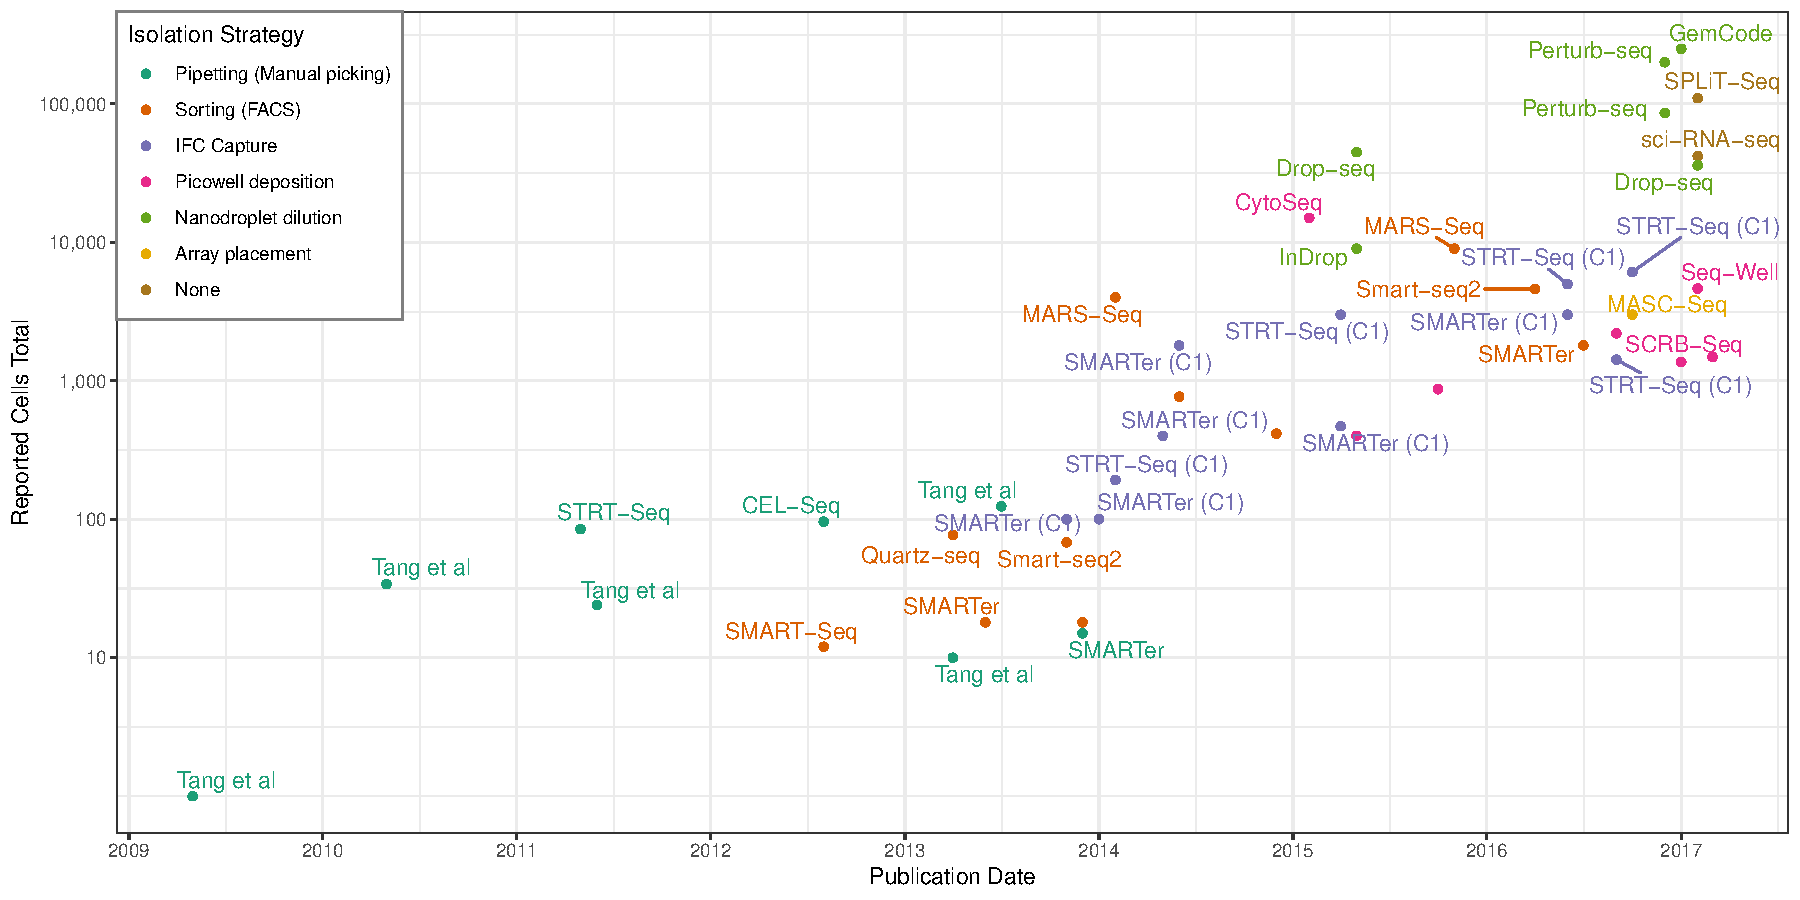
\includegraphics[width=0.85\textwidth]{figures/scRNATimeline.pdf} 
	\end{center}

	\blfootnote{Data taken from \cite{pmid29494575}}

\end{frame}

\begin{frame}{Droplet-based Approaches}

	\begin{center}
		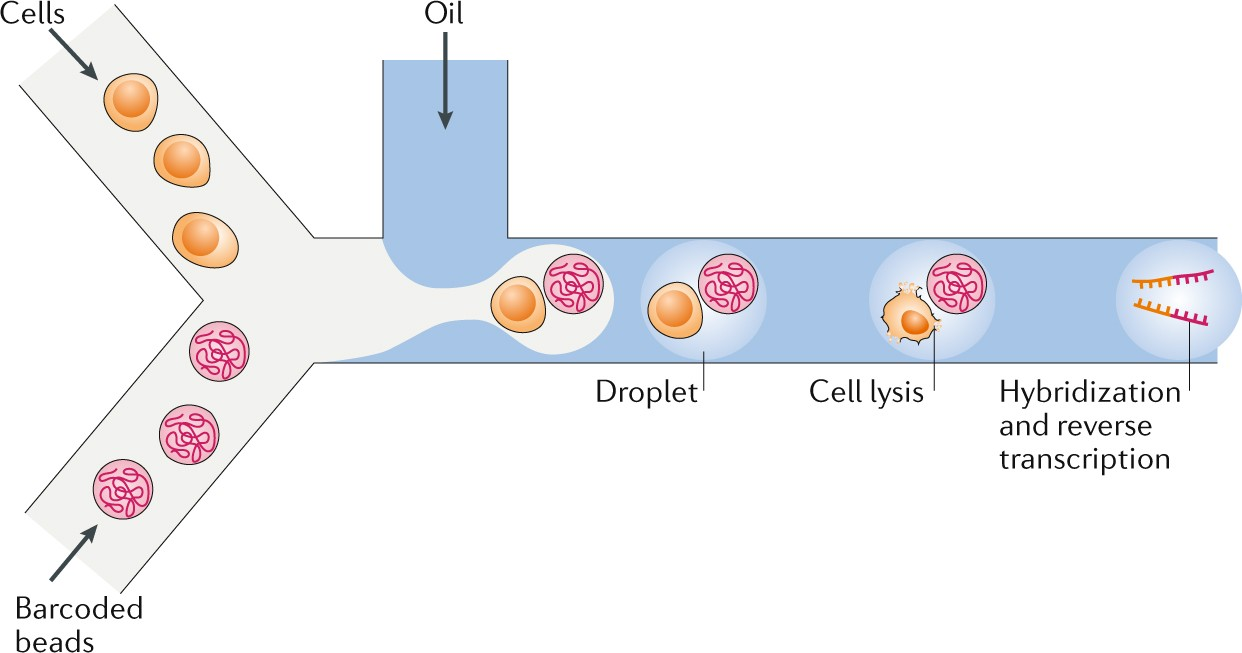
\includegraphics[width=0.7\textwidth]{figures/Droplet.jpg}
	\end{center}
	
	\pause
	Flow rate is modelled as a \textit{Poisson} process to minimise doublets
	
	\blfootnote{Taken from \cite{pmid29789704}}

\end{frame}

\subsection{Sequencing Protocols}

\begin{frame}{Sequencing Overview}

	\begin{itemize}
		\item Individual cells are isolated $\implies$ how do we sequence?
		\item Need a method to track which reads come from which cell
		\item Sequencing is performed on a standard Illumina machine, i.e. multiplexed
		\item Each cell is essentially an individual library prep
		\begin{itemize}
			\item Barcodes / UMIs are used for cell / molecule identification
		\end{itemize}
		\item For bulk RNA-Seq we need $0.1-1\mu$g of RNA ($10^5-10^6$pg)
		\begin{itemize}
			\item An individual cell contains 1-50pg
		\end{itemize}
	\end{itemize}

\end{frame}

\begin{frame}{SMART\footnote{SMART = Switching Mechanism at 5' End of RNA Template}-Seq (C1)}

	\begin{enumerate}
		\item All reagents are in the IFC reaction chambers
		\item Cells are lysed
		\item polyA RNA reverse transcribed into \textbf{full length cDNA}
		\begin{itemize}
			\item oligo(dT) priming and template switching
		\end{itemize}
		\item 12-18 PCR cycles
		\item cDNA fragmentation and Adapter ligation
	\end{enumerate}


\end{frame}

\begin{frame}
	\begin{center}
	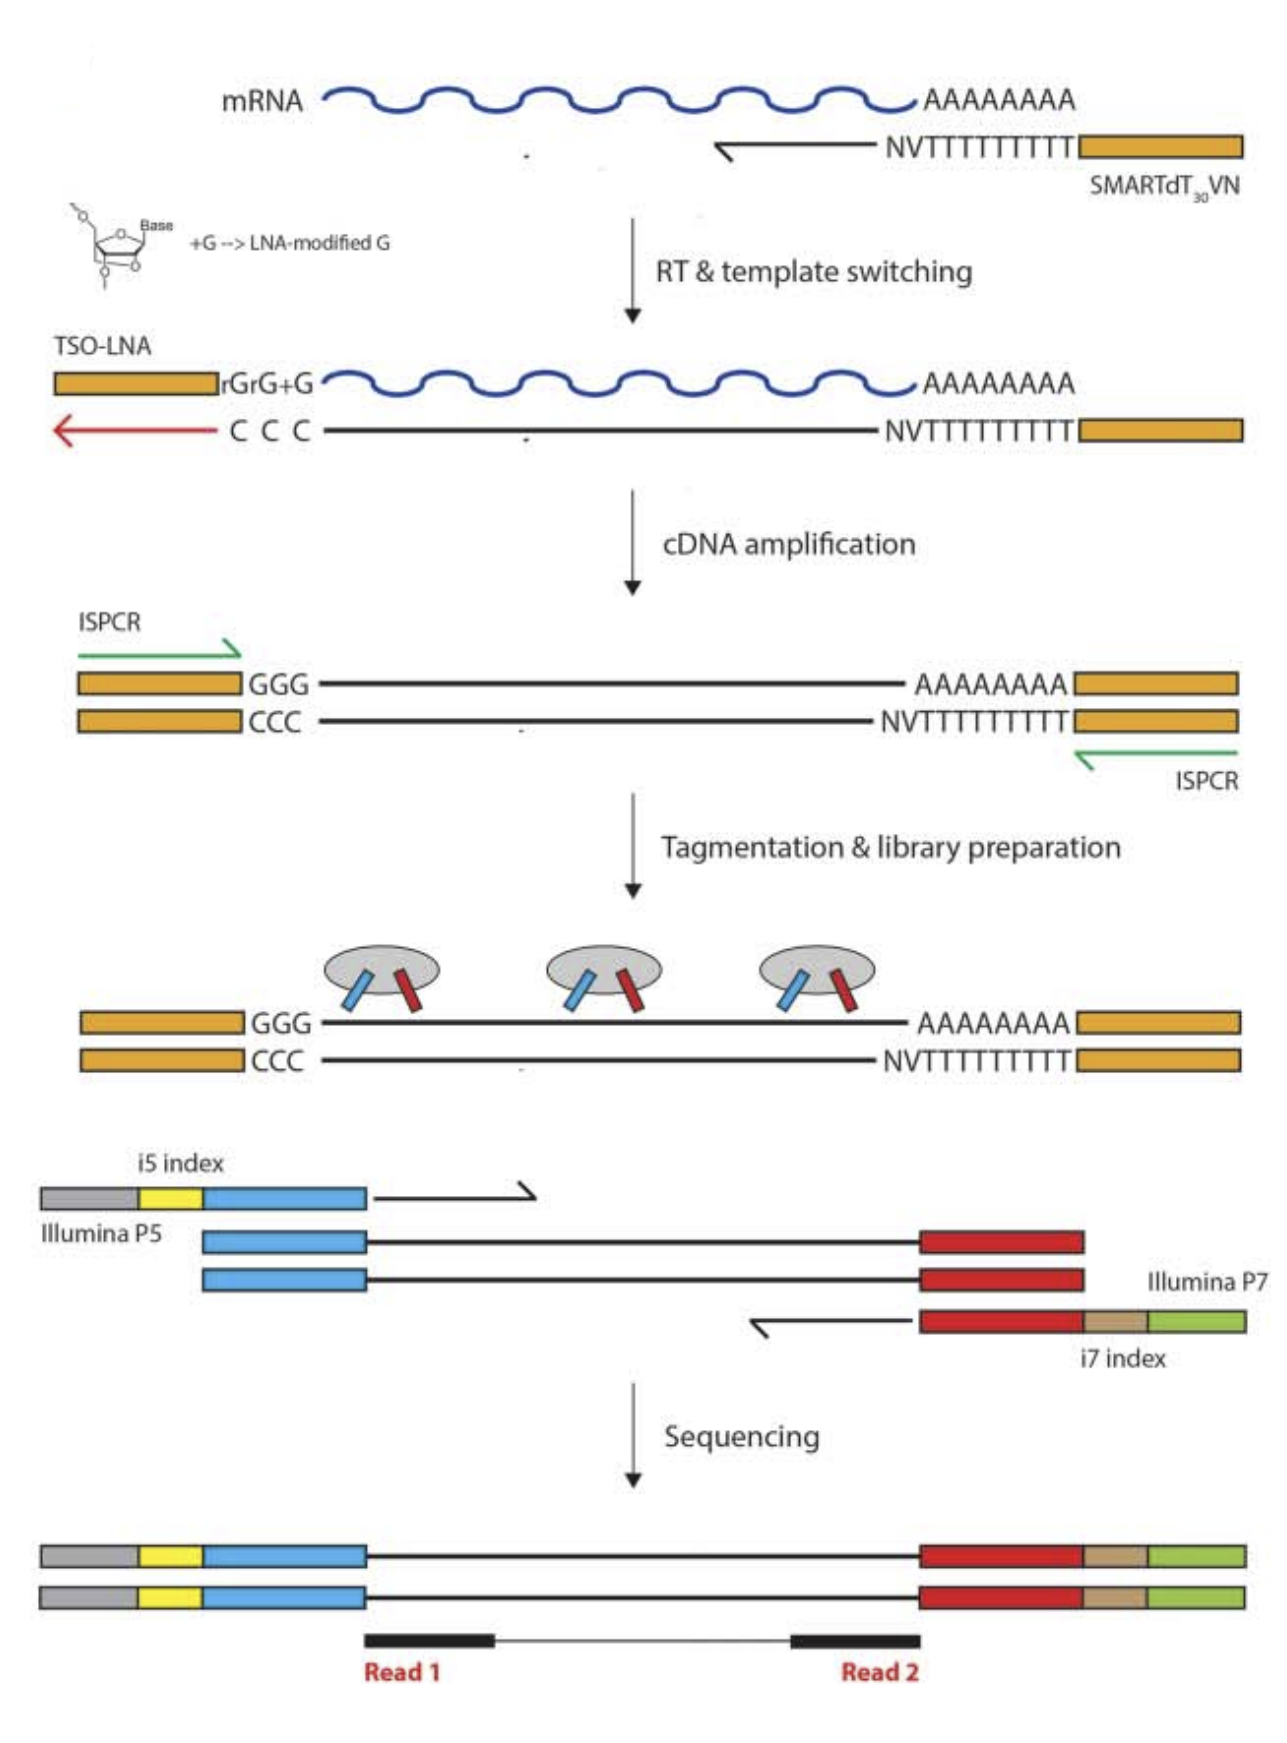
\includegraphics[width=0.35\textwidth]{figures/SMARTSeq.png} 
	\end{center}
	\blfootnote{Image from \cite{pmid27442339}}
\end{frame}

\begin{frame}{Droplet-based Methods}

	\begin{itemize}
		\item Popularised by the 10X Genomics Chromium System
		\item Each gel bead contains the reagents
		\begin{itemize}
			\item 30nt poly(dT) primer with 16nt 10x Barcode, 12nt UMI\footnote{Unique Molecular Identifier}
		\end{itemize}
		\item Illumina primers and restriction enzymes added later
	\end{itemize}

\end{frame}

\begin{frame}{10X Chromium Protocol}

	\begin{columns}[T]
		\begin{column}{.45\textwidth}
			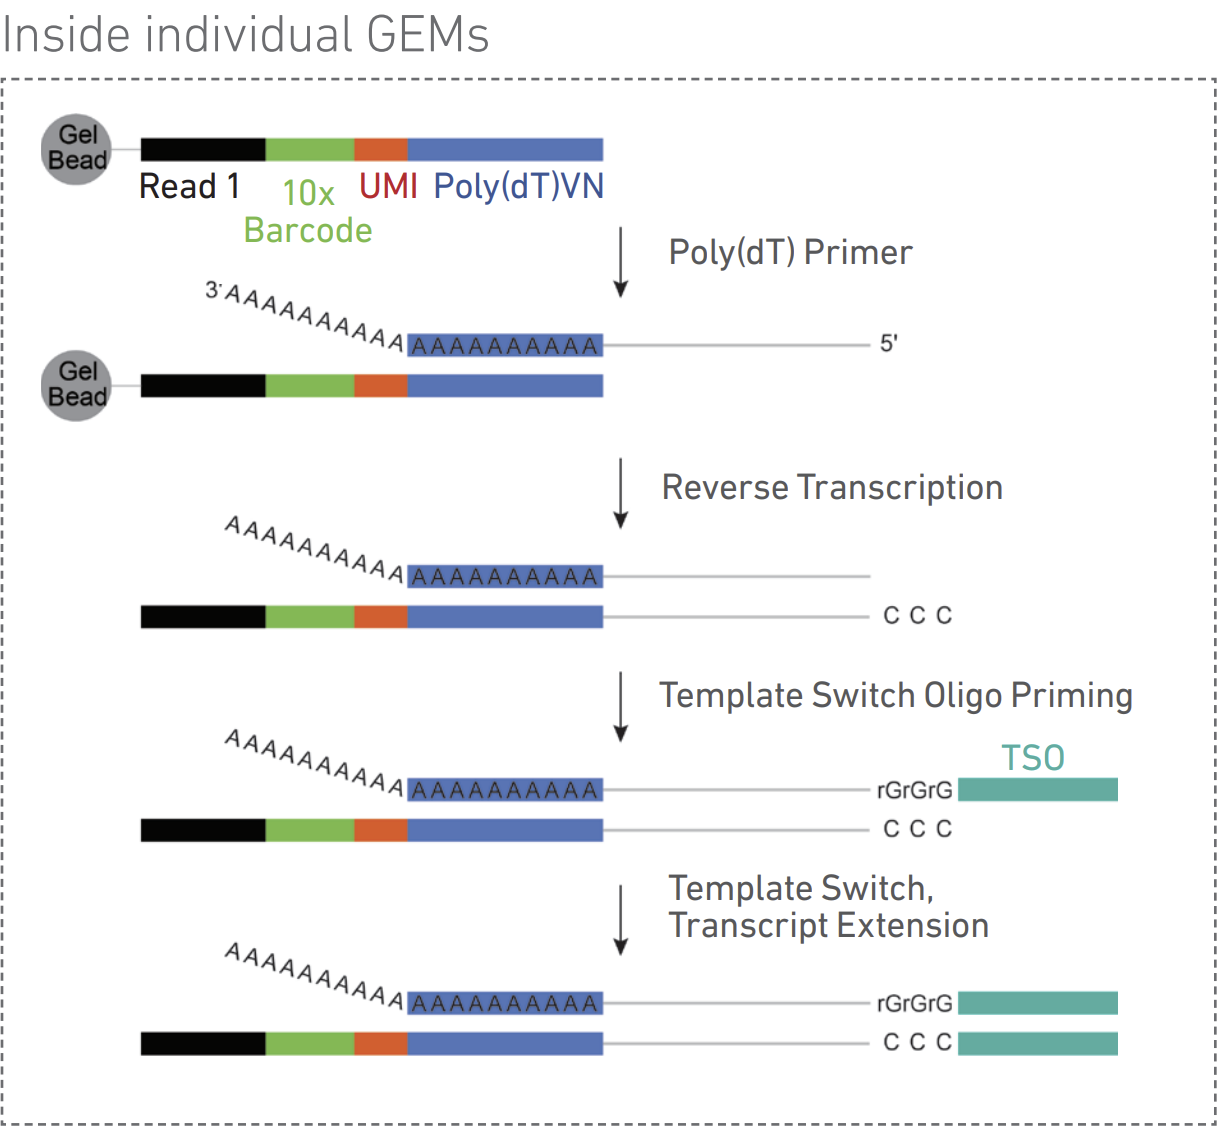
\includegraphics[width=0.75\textwidth]{figures/10xInsideGEM.png} 
			~\\[3mm]
			\small
			Barcoded, full-length cDNA is pooled then PCR amplified
		\end{column}
		\hfill
		\pause
		\begin{column}{.45\textwidth}
			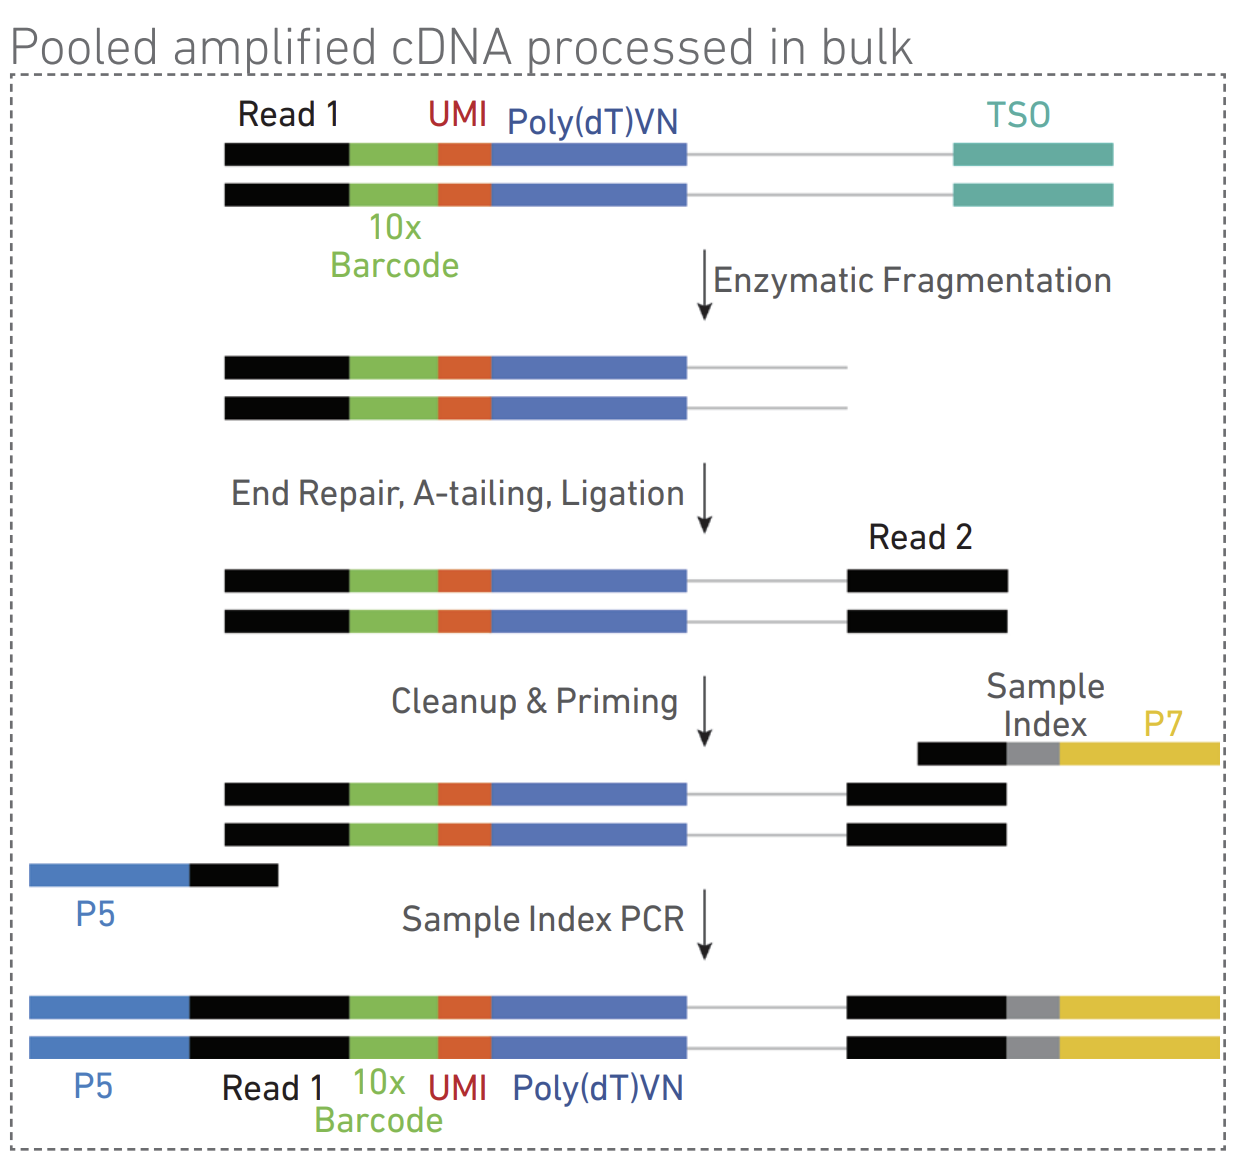
\includegraphics[width=0.75\textwidth]{figures/10xPooled.png} 
		\end{column}
	\end{columns}
	\blfootnote{Images from \href{https://assets.ctfassets.net/an68im79xiti/1eX2FPdpeCgnCJtw4fj9Hx/7cb84edaa9eca04b607f9193162994de/CG000204\_ChromiumNextGEMSingleCell3\_v3.1\_Rev\_D.pdf}{10X Genomics CG000204\_ChromiumNextGEMSingleCell3\_v3.1\_Rev\_D.pdf}}
\end{frame}

\begin{frame}{10X Chromium Protocol}
	\begin{center}
		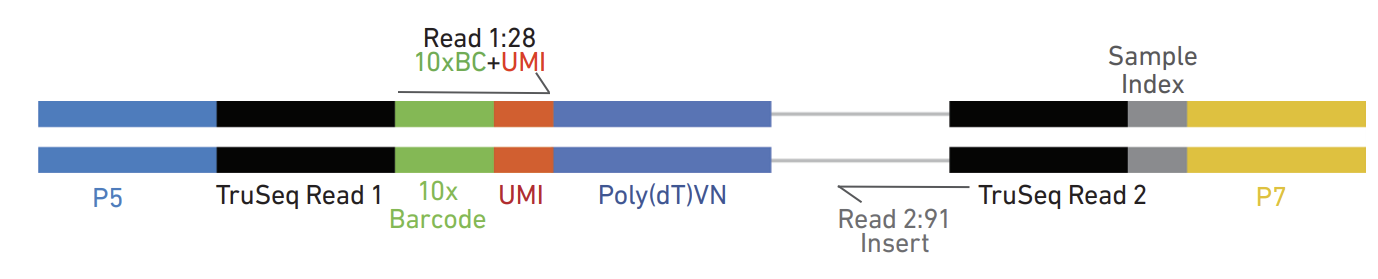
\includegraphics[width=0.6\textwidth]{figures/10XPairedRead.png} 
	\end{center}
	
	\begin{itemize}
		\item Only R2 contains the sequence information
		\item Only the 3' end is sequenced
		\item Each template RNA should have one UMI $\implies$ PCR duplicates can be identified
	\end{itemize}		
	
\end{frame}

\begin{frame}{Other Variations}

CITE-Seq\footnote{Cellular Indexing of Transcriptomes and Epitopes by sequencing}
	
	\begin{itemize}
		\item Prior to sorting cells can be `labelled' with antibody-oligo complexes
		\item Oligos allow additional recognition of surface proteins
		\item On cell lysis these oligos are amplified along with RNA
	\end{itemize}		
	
\end{frame}

\begin{frame}{Other Variations}

SPLIT-Seq\footnote{Split-Pool Ligation-based Transcriptome Sequencing}
	\begin{itemize}
		\item Cells are split into pools and fixed
		\item One barcode/pool
		\item Multiple rounds of pooling and barcoding
		\item All amplification is \textit{in situ}
		\item Able to be applied to single nuclei
	\end{itemize}
	
\end{frame}

\begin{frame}{Comparison of Methods}

	\begin{center}
	
		\small
		\begin{tabular}{l|llll}
			\textbf{Protocol} & \textbf{C1 (SMART-Seq)} & \textbf{SMART-Seq2} & \textbf{Chromium} & \textbf{SPLIT-Seq}\\
			\midrule
			\textit{Platform} & Microfluidics & Plate-based & Droplet & Plate-based\\
			\textit{Transcript} & Full-length & Full-length & 3'-end & 3'-end\\
			\textit{Cells} & $10^2 - 10^3$ & $10^2 - 10^3$ & $10^3-10^4$ & $10^3 - 10^5$\\
			\textit{Reads/Cell} & $10^6$ & $10^6$ & $10^4-10^5$ & $10^4$\\
			\bottomrule
		\end{tabular}

	\end{center}

	\blfootnote{Data sourced from \cite{pmid28821273}}

\end{frame}

\begin{frame}{Protocol Timeline}

	\begin{center}
		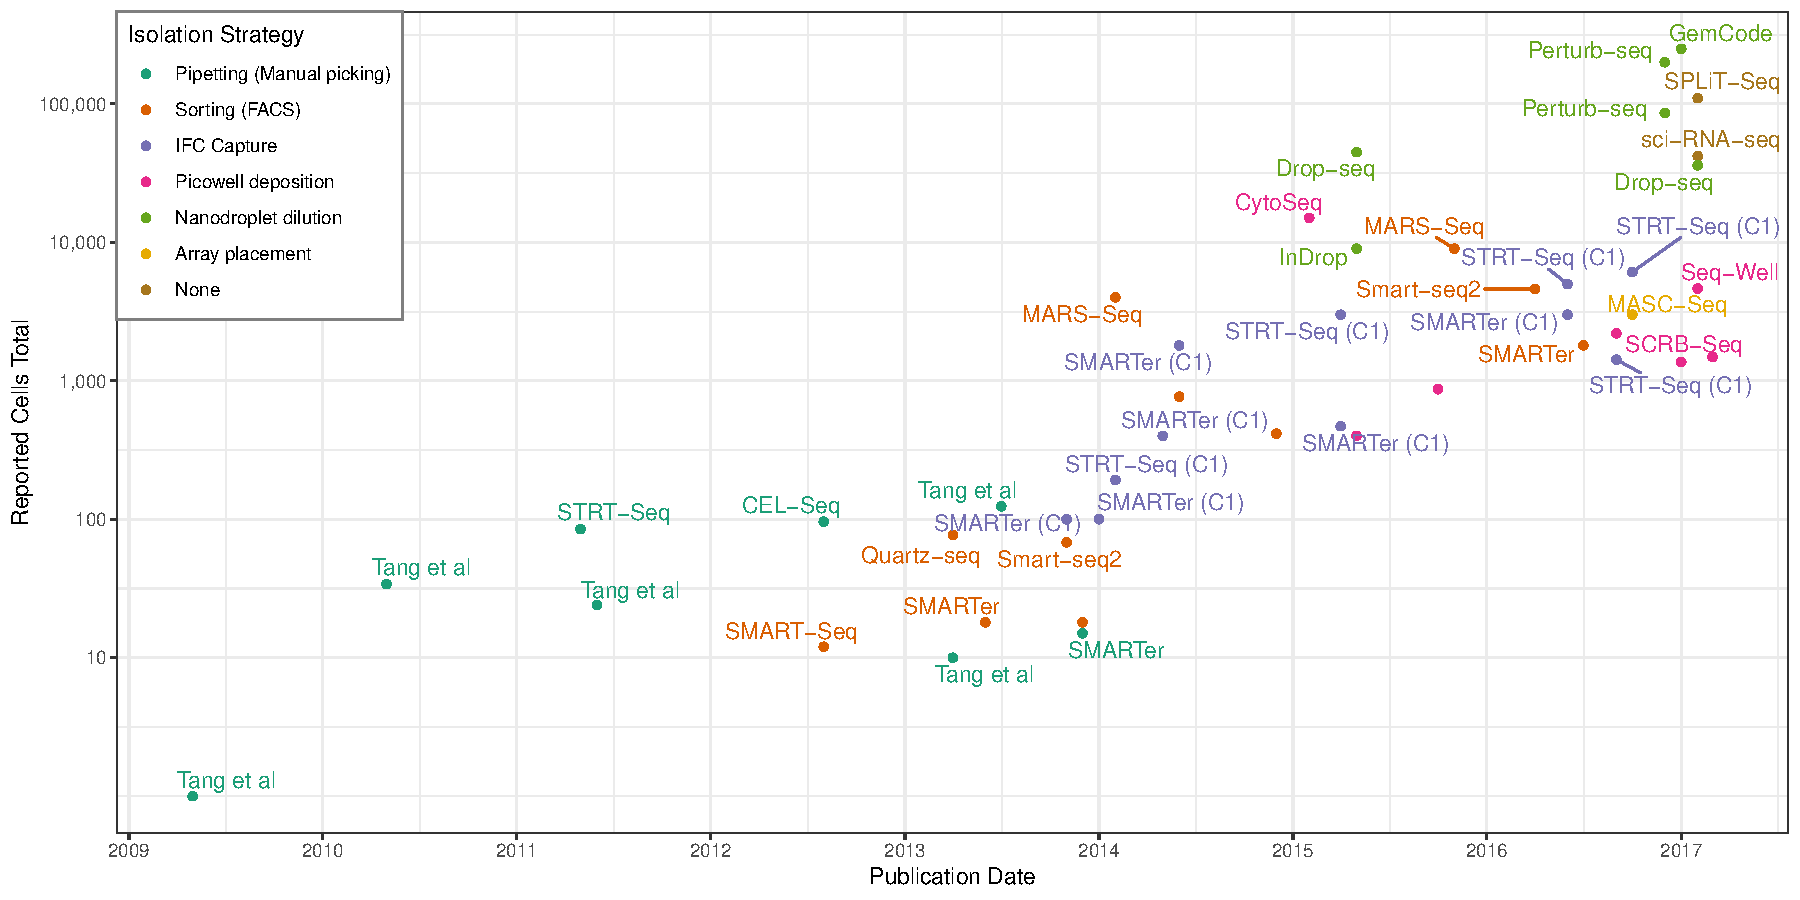
\includegraphics[width=0.85\textwidth]{figures/scRNATimeline.pdf} 
	\end{center}

	\blfootnote{Data taken from \cite{pmid29494575}}

\end{frame}


\section{Data Analysis}

\subsection{QC}

\subsection{Quantification}

\subsection{Normalisation}

\subsection{Clustering}

\subsection{DE Analysis}

\subsection{Trajectory Analysis}

\section{Spatial Transcriptomics}


\end{document}
